\documentclass[../../main]{subfiles}
\begin{document}
\newpage
\subsection{Recommendation from the app}
\label{ss:final-recommendation}
The recommendation section is the most important of the whole app considering the social/context aware part.
It is build to recommend some place to the user, when he enters in a geofence or after a certain amount of time.
The context aware part is managed from the model that can predict a category thanks to the information in input and retrieve the nearest point of that category 
to deliver it to the user. Instead the social aware part is made by searching the nearest point not only in the user's list but also in the publics pois of all
of his friends giving more context to the recommendation.
When a place of the right category is found the server send a push notification to the client and after the click show the detail of that poi 
asking the user for a feedback as shown in the next figure:
\begin{figure}[H]
    \centering
    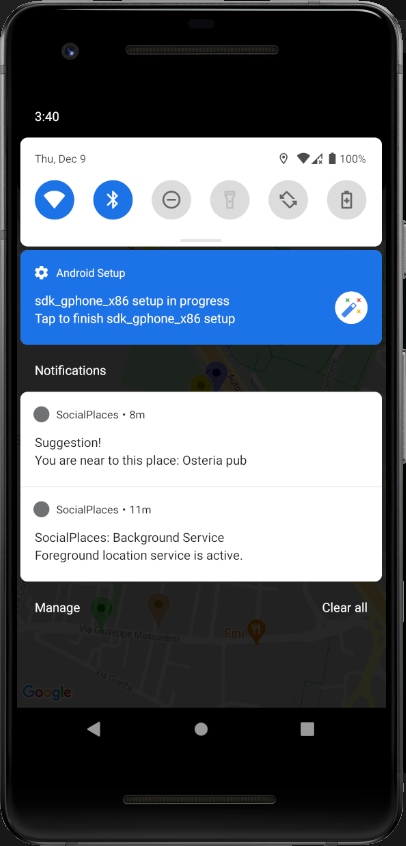
\includegraphics[width=70mm,height=150mm]{images/app/notification/recommendation/recommendation_request.png}
    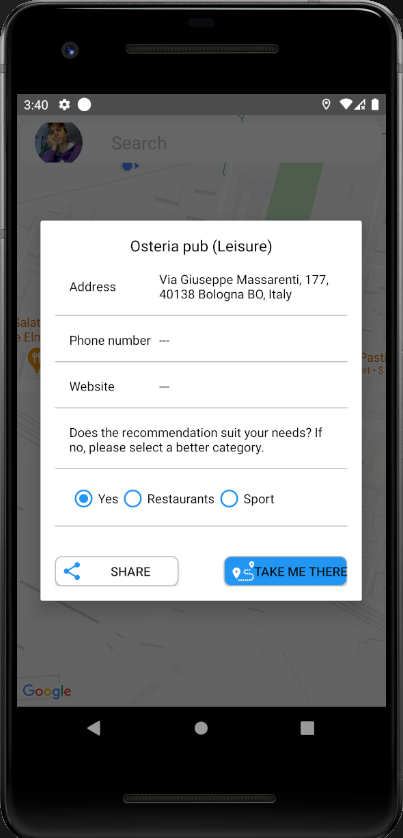
\includegraphics[width=70mm,height=150mm]{images/app/notification/recommendation/user_feedback.png}
    \caption{On the left the notification of place recommended and on the right the dialog for the user's feedback.}
\end{figure}

When the user close the feedback's dialog a new request is maid to retrain the model and after that a notification is sent with the new accuracy.
\begin{figure}[H]
    \centering
    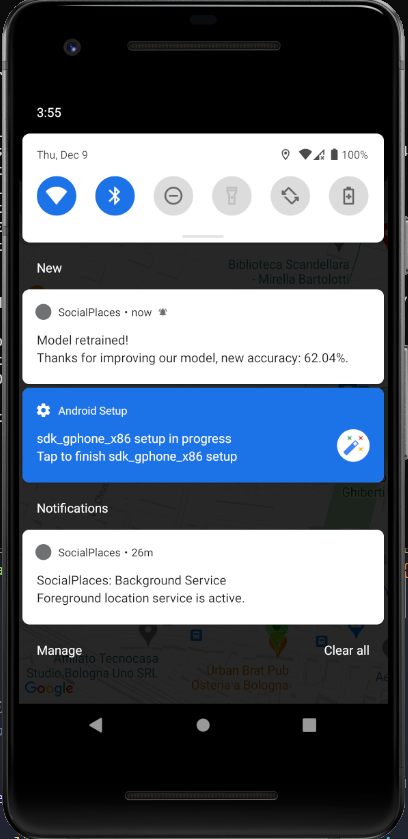
\includegraphics[width=70mm,height=150mm]{images/app/notification/recommendation/new_accuracy.png}
    \caption{Model retrained notification.}
\end{figure}
\end{document}